\documentclass[tikz,border=10pt]{standalone}
\usepackage{tikz}
\usetikzlibrary{arrows.meta,positioning}
\usetikzlibrary{positioning}
\usetikzlibrary{shapes.geometric}

\begin{document}

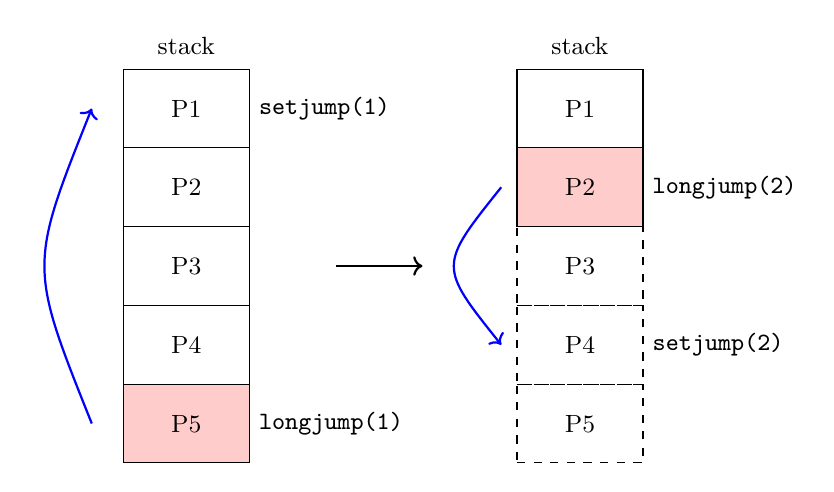
\begin{tikzpicture}[font=\small]

% ==== Left Stack ====
\node at (-2,4.8) {stack};

% Draw stack frames (left)
\foreach \name/\y in {P1/4, P2/3, P3/2, P4/1, P5/0}
    \node[draw, minimum width=1.6cm, minimum height=1cm] (L\name) at (-2,\y) {\name};

% Highlight P5
\node[draw, minimum width=1.6cm, minimum height=1cm, fill=red!20] (LP5) at (-2,0) {P5};

% setjump(1)
\draw (-1.2,4) node[right]{\texttt{setjump(1)}};

% longjump(1)
\draw (-1.2,0) node[right]{\texttt{longjump(1)}};

% Curved arrow left
\draw[->, thick, blue] (-3.2,0) .. controls (-4,2) .. (-3.2,4);


% ===== Arrow to right side =====
\draw[->, thick] (-0.1,2) -- (1.0,2);


% ==== Right Stack ====
\node at (3,4.8) {stack};

% Right stack frames (solid)
\node[draw, minimum width=1.6cm, minimum height=1cm] (RP1) at (3,4) {P1};
\node[draw, minimum width=1.6cm, minimum height=1cm, fill=red!20] (RP2) at (3,3) {P2};

% Dashed frames
\foreach \name/\y in {P3/2, P4/1, P5/0}
    \node[draw, dashed, minimum width=1.6cm, minimum height=1cm] (R\name) at (3,\y) {\name};

% longjump(2)
\draw (3.8,3) node[right]{\texttt{longjump(2)}};

% setjump(2)
\draw (3.8,1) node[right]{\texttt{setjump(2)}};

% Curved arrow right
\draw[->, thick, blue] (2,3) .. controls (1.2,2) .. (2,1);

\end{tikzpicture}

\newpage

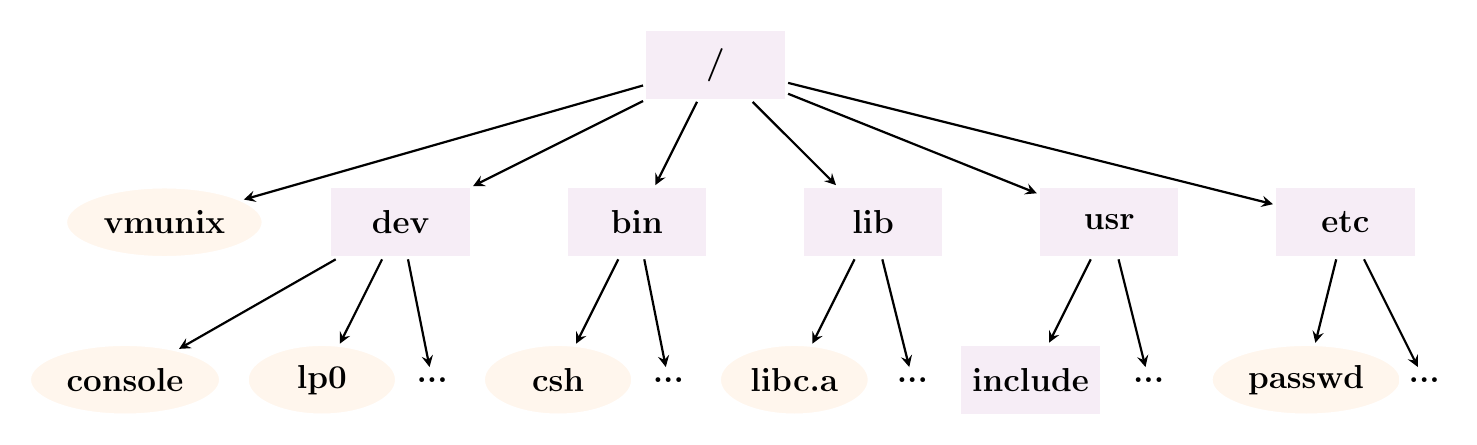
\begin{tikzpicture}[
    x=1cm,y=1cm,
    >=stealth,
    text=white,
    thick,
    box/.style={
        draw=white, very thick,
        rectangle,
        fill=violet!7,
        minimum width=1.8cm,
        minimum height=0.9cm,
        align=center,
        font=\bfseries\large,
        text=black
    },
    oval/.style={
        draw=white, very thick,
        ellipse,
        fill=orange!7,
        minimum width=1.9cm,
        minimum height=0.9cm,
        align=center,
        font=\bfseries\large,
        text=black
    },
    dir/.style={
        draw=none,
        fill=white,
        text=black,
        align=center,
        font=\bfseries\large
    }
]

% ====== 上層節點 ======
\node[box] (root) at (0,0) {/};

\node[box] (dev) at (-4,-2) {dev};
\node[box] (bin) at (-1,-2) {bin};
\node[box] (lib) at ( 2,-2) {lib};
\node[box] (usr) at ( 5,-2) {usr};
\node[box] (etc) at ( 8,-2) {etc};

\node[oval] (vmunix) at (-7,-2) {vmunix};

% root → 第一層
\draw[->] (root) -- (dev);
\draw[->] (root) -- (bin);
\draw[->] (root) -- (lib);
\draw[->] (root) -- (usr);
\draw[->] (root) -- (etc);
\draw[->] (root) -- (vmunix); % 長斜箭頭到 vmunix

% ====== 第二層:dev 下方 ======
\node[oval] (console) at (-7.5,-4) {console};
\node[oval] (lp0)     at (-5.0,-4) {lp0};
\node[dir] (devdot)  at (-3.6,-4) {...};

\draw[->] (dev) -- (console);
\draw[->] (dev) -- (lp0);
\draw[->] (dev) -- (devdot);

% ====== 第二層:bin 下方 ======
\node[oval] (csh)    at (-2.0,-4) {csh};
\node[dir] (bindot) at ( -0.6,-4)  {...};

\draw[->] (bin) -- (csh);
\draw[->] (bin) -- (bindot);

% ====== 第二層:lib 下方 ======
\node[oval] (libca)   at (1.0,-4) {libc.a};
\node[dir] (libdot)  at (2.5,-4) {...};

\draw[->] (lib) -- (libca);
\draw[->] (lib) -- (libdot);

% ====== 第二層:usr 下方 ======
\node[box] (include)  at (4.0,-4) {include};
\node[dir] (usrdot)   at (5.5,-4) {...};

\draw[->] (usr) -- (include);
\draw[->] (usr) -- (usrdot);

% ====== 第二層:etc 下方 ======
\node[oval] (passwd)  at (7.5,-4) {passwd};
\node[dir] (etcdot)  at (9.0,-4) {...};

\draw[->] (etc) -- (passwd);
\draw[->] (etc) -- (etcdot);

\end{tikzpicture}

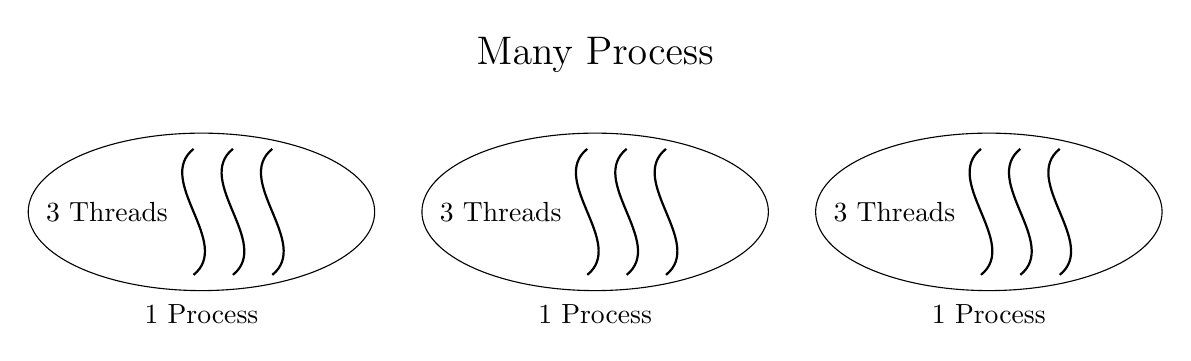
\begin{tikzpicture}[>=stealth, x=1cm, y=1cm]

% Macro: Draw one flattened ellipse with wavy threads
\newcommand{\processthreads}[2]{
\begin{scope}[shift={(#1,0)}]

    % Flattened ellipse
    \draw (0,0) ellipse (2.2cm and 1.0cm);

    % MANY wavy threads inside
    \foreach \x in {-0.1, 0.4, 0.9} {
        \draw[thick]
            (\x,-0.8)
                .. controls (\x+0.5,-0.4) and (\x-0.5,0.4) ..
            (\x,0.8);
    }
    \node at (-1.2, 0) {3 Threads};
    % Label
    \node at (0,-1.3) {#2};

\end{scope}
}

% Draw 3 side-by-side thread groups
\processthreads{-5}{1 Process}
\processthreads{0}{1 Process}
\processthreads{5}{1 Process}

% Optional title
\node at (0,2) {\Large Many Process};

\end{tikzpicture}

\newpage

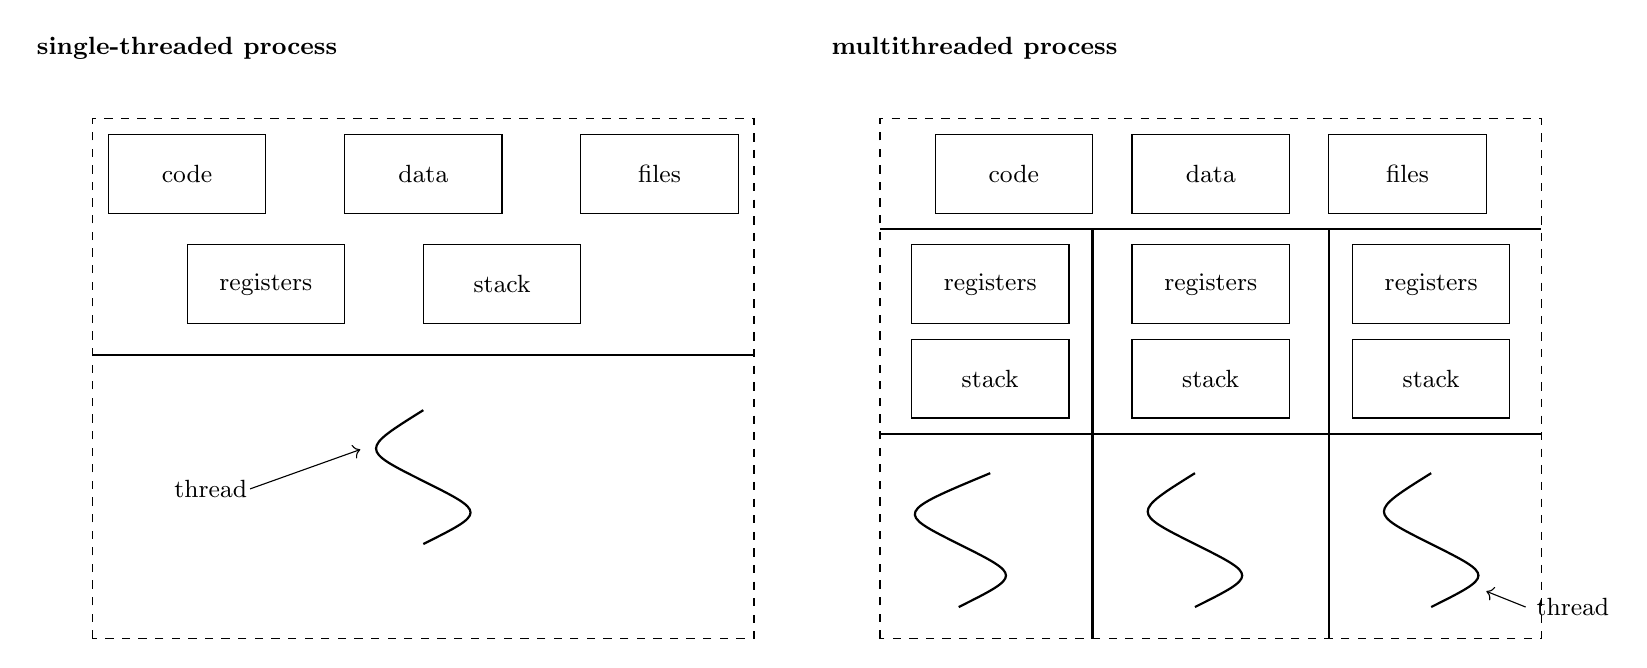
\begin{tikzpicture}[font=\small]

% ===============================================================
% Left: Single-threaded
% ===============================================================

\node at (0,4.2) {\bf single-threaded process};

% dashed outer box
\draw[dashed] (-1.2,-3.3) rectangle (7.2,3.3);

% Top row: code/data/files
\node[draw, minimum width=2cm, minimum height=1cm] (lcode)  at (0,2.6) {code};
\node[draw, minimum width=2cm, minimum height=1cm] (ldata)  at (3,2.6) {data};
\node[draw, minimum width=2cm, minimum height=1cm] (lfiles) at (6,2.6) {files};

% registers + stack row
\node[draw, minimum width=2cm, minimum height=1cm] (lreg)   at (1,1.2) {registers};
\node[draw, minimum width=2cm, minimum height=1cm] (lstack) at (4,1.2) {stack};

% horizontal separator line
\draw[thick] (-1.2,0.3) -- (7.2,0.3);

% Single thread squiggle (3-wave curve)
\draw[thick]
    (3,-0.4) .. controls (2.2,-0.9) .. (3,-1.3)
            .. controls (3.8,-1.7) .. (3,-2.1);

\node at (0.3,-1.4) {thread};
\draw[->] (0.8,-1.4) -- (2.2,-0.9);

% ===============================================================
% Right: Multithreaded
% ===============================================================

\begin{scope}[xshift=10cm]

\node at (0,4.2) {\bf multithreaded process};

% dashed outer box
\draw[dashed] (-1.2,-3.3) rectangle (7.2,3.3);

% Top row: code/data/files
\node[draw, minimum width=2cm, minimum height=1cm] (rcode)  at (0.5,2.6) {code};
\node[draw, minimum width=2cm, minimum height=1cm] (rdata)  at (3,2.6) {data};
\node[draw, minimum width=2cm, minimum height=1cm] (rfiles) at (5.5,2.6) {files};

\draw[thick] (-1.2, 1.9) -- (7.2, 1.9);

% Registers rows
\node[draw, minimum width=2cm, minimum height=1cm] (rreg1) at (0.2,1.2) {registers};
\node[draw, minimum width=2cm, minimum height=1cm] (rreg2) at (3,1.2) {registers};
\node[draw, minimum width=2cm, minimum height=1cm] (rreg3) at (5.8,1.2) {registers};

% Stacks
\node[draw, minimum width=2cm, minimum height=1cm] (rstack1) at (0.2,0) {stack};
\node[draw, minimum width=2cm, minimum height=1cm] (rstack2) at (3,0) {stack};
\node[draw, minimum width=2cm, minimum height=1cm] (rstack3) at (5.8,0) {stack};

% Vertical separators
\draw[thick] (1.5,1.9) -- (1.5,-3.3);
\draw[thick] (4.5,1.9) -- (4.5,-3.3);

% Horizontal separator line
\draw[thick] (-1.2,-0.7) -- (7.2,-0.7);

\def\threadY{-1.2}   % 你要的 thread y 起始位置

% First thread
\draw[thick]
    (0.2,\threadY) .. controls (-1,\threadY-0.5) .. (-0.2,\threadY-0.9)
                    .. controls (0.6,\threadY-1.3) .. (-0.2,\threadY-1.7);

% Second thread
\draw[thick]
    (2.8,\threadY) .. controls (2,\threadY-0.5) .. (2.8,\threadY-0.9)
                    .. controls (3.6,\threadY-1.3) .. (2.8,\threadY-1.7);

% Third thread
\draw[thick]
    (5.8,\threadY) .. controls (5,\threadY-0.5) .. (5.8,\threadY-0.9)
                    .. controls (6.6,\threadY-1.3) .. (5.8,\threadY-1.7);


% Thread arrow
\node at (7.6,\threadY-1.7) {thread};
\draw[->] (7,\threadY-1.7) -- (6.5,\threadY-1.5);

\end{scope}

\end{tikzpicture}

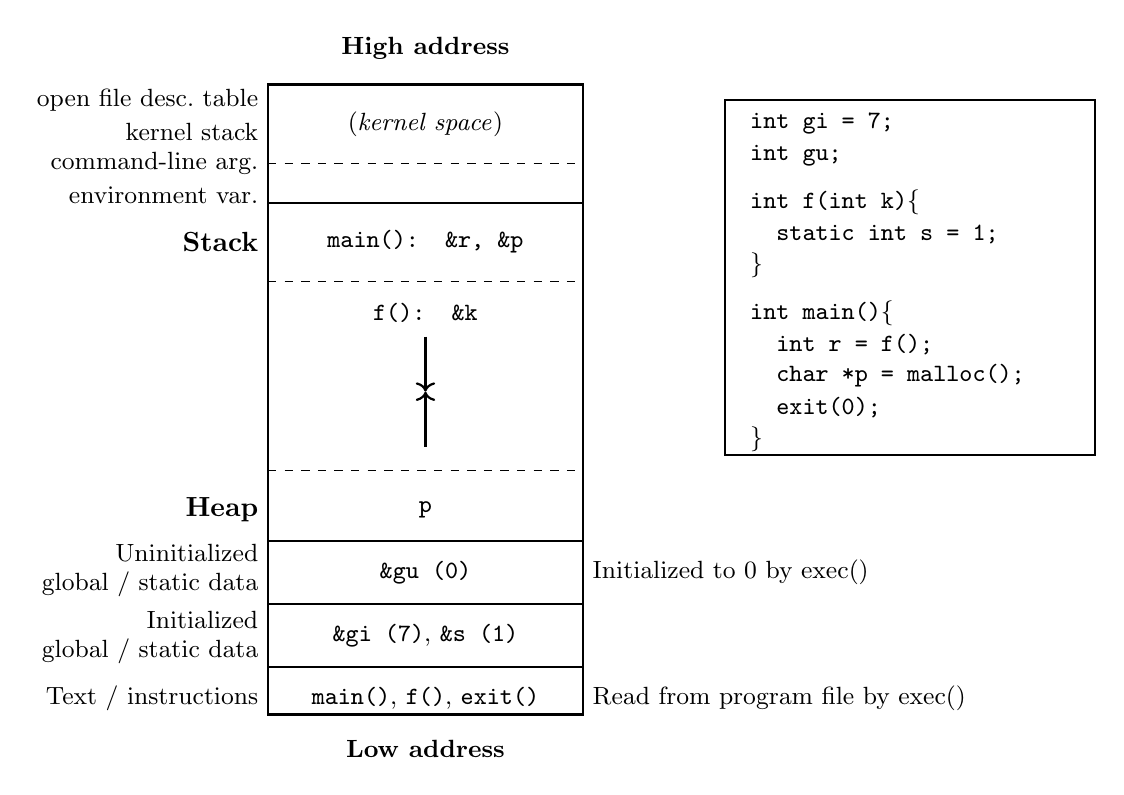
\begin{tikzpicture}[font=\small]

% ========================
% LEFT LABELS (aligned right to x=0)
% ========================

% Left labels baseline positions (re-aligned)
\node[anchor=east] at (0,3.8) {open file desc.\ table};
\node[anchor=east] at (0,3.4) {kernel stack};
\node[anchor=east] at (0,3.0) {command-line arg.};
\node[anchor=east] at (0,2.6) {environment var.};

\node[anchor=east,font=\bfseries] at (0,2.0) {Stack};

\node[anchor=east,font=\bfseries] at (0,-1.4) {Heap};

\node[anchor=east] at (0,-1.95) {Uninitialized};
\node[anchor=east] at (0,-2.35) {global / static data};

\node[anchor=east] at (0,-2.8) {Initialized};
\node[anchor=east] at (0,-3.2) {global / static data};

\node[anchor=east] at (0,-3.8) {Text / instructions};


% ========================
% MAIN MEMORY BLOCK
% ========================

\draw[thick] (0,4) rectangle (4,-4);

% kernel space
\node at (2,3.5) {(\textit{kernel space})};

\draw[dashed] (0,3.0) -- (4,3.0);

% main(): &r &p
\node at (2,2) {{\texttt{main(): \&r, \&p}}};
\draw[thick] (0,2.5) -- (4,2.5);

% f(): &k
\draw[dashed] (0,1.5) -- (4,1.5);
\node at (2,1.1) {{\texttt{f(): \&k}}};

% stack downward arrow
\draw[->,thick] (2,0.8) -- (2,0.1);
\draw[<-,thick] (2,0.1) -- (2,-0.6);

% heap p
\draw[dashed] (0,-0.9) -- (4,-0.9);
\node at (2,-1.4) {\texttt{p}};

\draw[thick] (0,-1.8) -- (4,-1.8);

% uninitialized global/static
\node at (2,-2.2) {\texttt{\&gu (0)}};
\draw[thick] (0,-2.6) -- (4,-2.6);

% initialized global/static
\node at (2,-3.0) {\texttt{\&gi (7)}, \texttt{\&s (1)}};
\draw[thick] (0,-3.4) -- (4,-3.4);

% text / instructions
\node at (2,-3.8) {\texttt{main()}, \texttt{f()}, \texttt{exit()}};

% Address labels
\node[anchor=south] at (2,4.2) {\bf High address};
\node[anchor=north] at (2,-4.2) {\bf Low address};


% ========================
% RIGHT CODE BLOCK (with border)
% ========================

\begin{scope}[xshift=7.5cm]

\draw[thick] (-1.7,3.8) rectangle (3,-0.7);  % code box frame

\node[anchor=west] at (-1.5,3.5) {\texttt{int gi = 7;}};
\node[anchor=west] at (-1.5,3.1) {\texttt{int gu;}};

\node[anchor=west] at (-1.5,2.5) {\texttt{int f(int k)\{}};
\node[anchor=west] at (-1.5,2.1) {\texttt{\ \ static int s = 1;}};
\node[anchor=west] at (-1.5,1.7) {\texttt{\}}};

\node[anchor=west] at (-1.5,1.1) {\texttt{int main()\{}};
\node[anchor=west] at (-1.5,0.7) {\texttt{\ \ int r = f();}};
\node[anchor=west] at (-1.5,0.3) {\texttt{\ \ char *p = malloc();}};
\node[anchor=west] at (-1.5,-0.1) {\texttt{\ \ exit(0);}};
\node[anchor=west] at (-1.5,-0.5) {\texttt{\}}};

% right-side comments
\node[anchor=west] at (-3.5,-2.2) {Initialized to 0 by exec()};
\node[anchor=west] at (-3.5,-3.8) {Read from program file by exec()};

\end{scope}

\end{tikzpicture}


\end{document}
